\section{Validation}\label{validation}

The aim of this step was to validate the utility of the tool with end users. To do this, we created a simple use case\footnote{\scriptsize{Experimentation package: \url{https://drive.google.com/file/d/0B3kzMiMYv9r2ZXZ2c2VsTnA4WWM/edit?usp=sharing}}}, and retrieve users impressions via a questionnaire\footnote{\scriptsize{Questionnaire: \url{https://docs.google.com/forms/d/1MUKfjnyXrpKdfKZ5nnhYtUxyO11aOrRDad5KT2DM-3g/viewform}}}.

\subsection{Use case}
\vspace{0.15em}
\noindent\textbf{Mind-mapping process.}
During this step, the user must create mind-map, inject the elements in the WordPress CMS, and then observe the changes of the website. The provided mind-map for this test consisted of four components, as shown in Fig.\ref{mindMapUseCase}: Post, Page, User and Theme. But the user was always able to add a element choosed among these four types.

			\begin{figure}[!h]
				\centering
				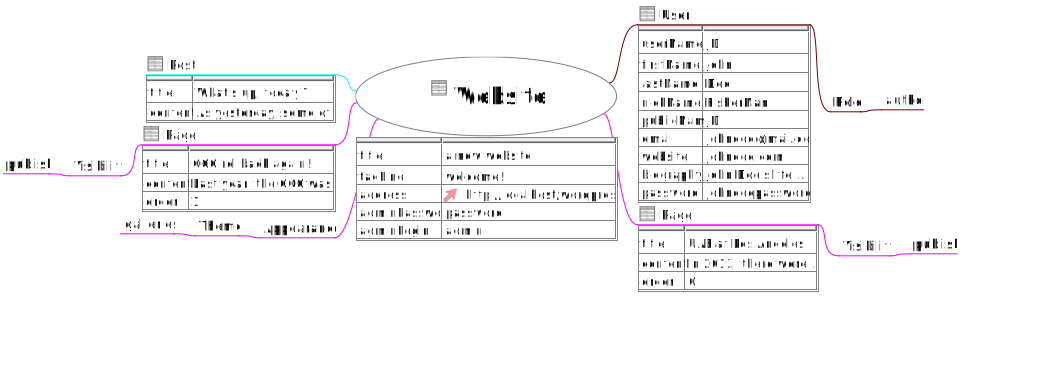
\includegraphics[width=\textwidth]{../resources/pdf/mindMapUseCase.pdf}
				\caption{Mind-map sample}
				\label{mindMapUseCase}
			\end{figure}

\vspace{0.15em}
\noindent\textbf{WordPress use.}
Users had to the same as in the previous step, but this time with WordPress, to be able to compare the two tools.

\vspace{0.15em}
\noindent\textbf{Comparison between WordPress and the mind-mapping process.}
Once both tools were used, users were able to give their opinion about the usefulness of a website configuration via a mind-mapping based DSL, by comparison to a tool such as WordPress.
	 
\subsection{Experimentation result}	 